%% SIGCHI Proceedings Format (modern) Sample Document
%% This sample file demonstrates the use of the `sigchi-modern' class file.
%%
%% The content of this document draws heavily on the `HCI Archive Format'
%% template supplied by SIGCHI, but has been modified to demonstrate and
%% document the LaTeX class.

% The parameter given to the `\documentclass' command can be one of:
%   `preprint', `submission', or `final'.
% These control the presence of certain features for each stage of the authoring
% process. For example, `submission' does not output the author block, and
% `final' disables page numbers.
%
% The \preprintonly{}, \submissiononly{}, and \finalonly{} commands allow you
% to wrap text that will only be output under the corresponding option.
%
\documentclass[preprint]{../latex/sigchi-modern}

% These packages aren't required, but do provide some helpful features that are
% used in this sample.
%
\usepackage{graphicx}  % Graphics for figures
\usepackage{booktabs}  % Nice formatting for tables
\usepackage{balance}   % Attempts to balance the columns on the last page

% A nice way to help avoid overful lines handing out into the margins is the
% `microtype' package, which lets certain characters extrude a *little* bit.
%
\usepackage{microtype}
% If the situation becomes dire, use:
%\sloppy

% You may use any bibliography package as long as the output matches that of
% the prescribed format. `natbib' is a fairly nice default, and the provided
% BibTeX style file has been tested with it.
%
\usepackage[square,comma,numbers,sort&compress]{natbib}
\bibliographystyle{../bibtex/acm-sigchi-modern}

% Define these tokens as appropriate for the conference to generate the
% necessary copyright notice for `final` mode.
%
\confname{CHI'14}
\confdate{April 26--May 1}
\confyear{2014}
\conflocation{Toronto, Canada}
\procissn{XXX-X-XXXX-XXXX-X/XX/XX}
\doi{10.1000/182}
% \copylicense be set to one of: \acmcopyright, \authorlicense, or \openlicense
\copylicense{\authorlicense}

% End of preamble. Here comes the document.
\begin{document}

\title{SIGCHI Conference Proceedings Format}

% Author information can be set automatically if you provide a series of
% author names and affiliations:
%   \author[1]{Author One}
%   \author[2]{Author Two}
%   \author[1,2]{Author Three}
%   \affiliation[1]{Organisation One\\
%                   Some Country}
%   \affiliation[2]{Organisation Two\\
%                   Some Country}
%   \authorextra{\mailto{one@example.com}, \mailto{two@example.org},
%                \mailto{three@example.net}}
% Or manually:
%   \author{
%     \authorname{Author One}\\
%     \authoraffil{
%       Organisation One\\
%       Some Country\\
%       \mailto{one@example.com}}}
%   \author{
%     \authorname{Author Two}\\
%     \authoraffil{
%       Organisation Two\\
%       Some Country\\
%       \mailto{two@example.org}}}
% Refer to the body text of the document for more details.
%
\author[1]{Author One}
\author[2]{Author Two}
\author[1]{Author Three}
\author[1,2]{Author Four}
% Set \authorwidth with the longest author name if you don't like the default
% spacing
%\settowidth{\authorwidth}{Author Three}

\affiliation[1]{Department of Examples\\
    Sample University\\
    City, Country}
\affiliation[2]{Sample Corporation\\City, Country}

\authorpostscript{\email{\{%
  \href{mailto:one@example.com}{one},
  \href{mailto:two@example.com}{two},
  \href{mailto:four@example.com}{four}\}@example.com},
  \mailto{three@example.org}}

% If you do the author blocks manually, you should use \authorlist to set a
% comma-delimited list of the author names.
% This is written into the PDF metadata for preprint and final modes.
%\authorlist{Author One, Author Two, Author Three, Author Four}

% A `banner' figure can appear below the affiliation block and above the main
% body of the paper. This banner spans two columns and is numbered and labelled
% as a regular figure.
\banner{
  \centering
  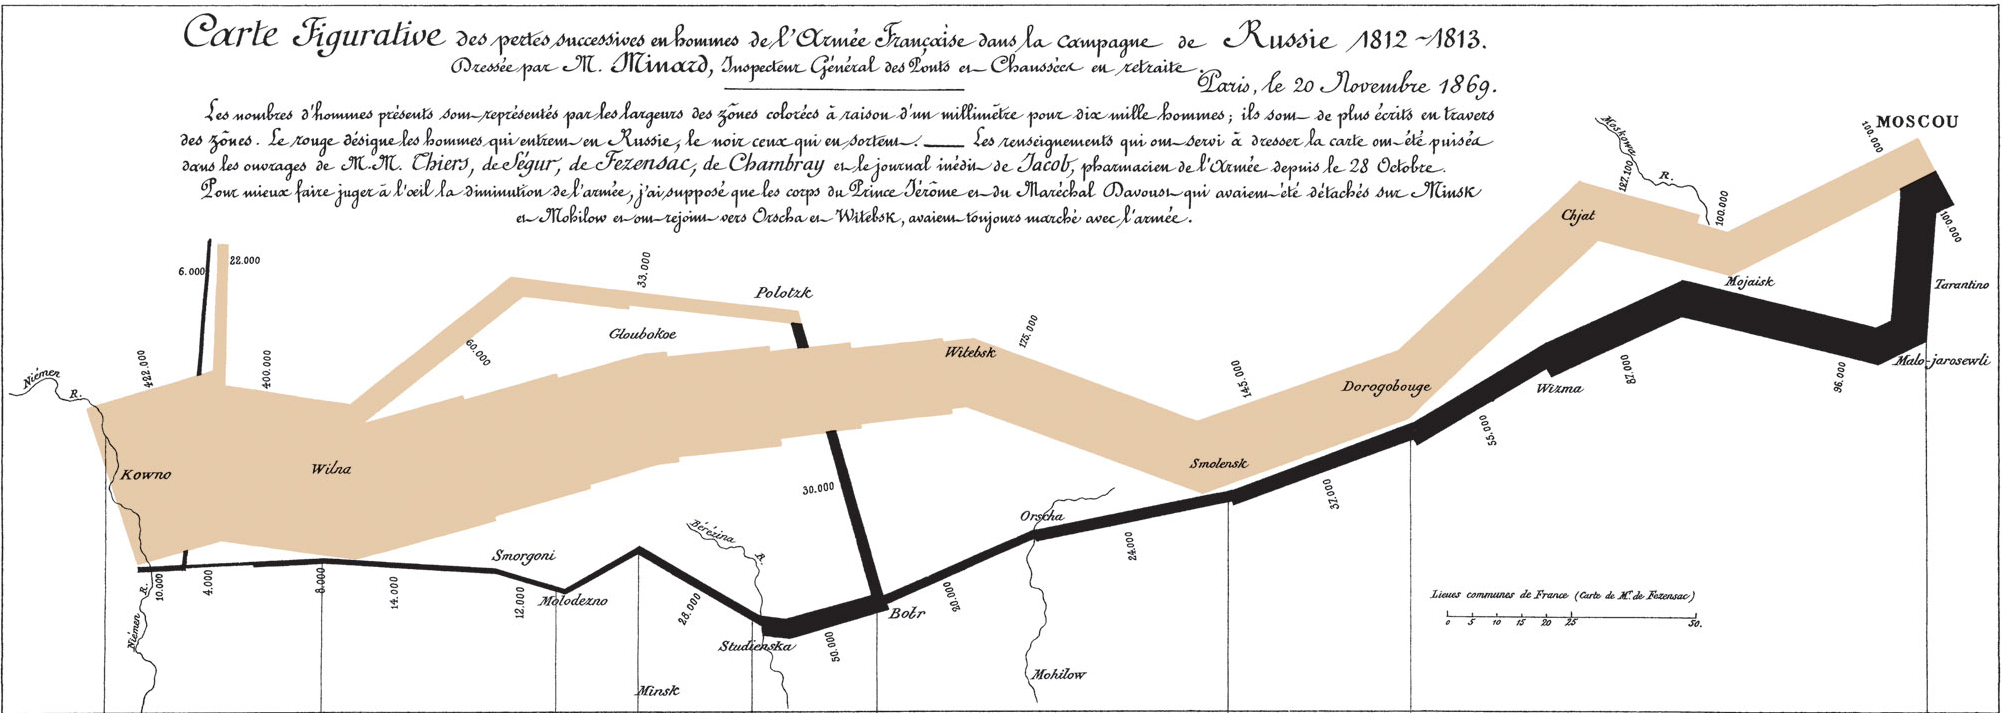
\includegraphics[width=\textwidth]{Minard}
  \caption{Example banner image spanning both columns. This command must be
           used before \texttt{\textbackslash maketitle}. In the remainder of
           the document, use the \texttt{\{figure*\}} environment to produce
           these.}
  \label{fig:banner}
}

% Produces the title, author, and optional banner block.
\maketitle

\begin{abstract}
This paper describes the formatting requirements for SIGCHI Conference
Proceedings and a few recommendations on writing for the worldwide SIGCHI
readership. This paper is also the documentation for the \LaTeX\ class
for producing formatted papers.
(This paper is not produced by SIGCHI, nor is it an authoritative source for
the described formatting.)
\end{abstract}

% This should be a semicolon-separated list of keywords to describe the paper.
\keywords{Guides; instructions; author's kit; conference publications.}

% This formats the ACM classification block.
% \category{}{}{}[] has three mandatory arguments and one optional argument; it
% can be used multiple times.
\classification{
    \category{H.5.m}{Information Interfaces and Presentation}{Miscellaneous}
}

\section{Introduction}
This format is to be used for submissions to SIGCHI conference proceedings. We
wish to give this volume a consistent, high-quality appearance, and therefore
ask that authors follow some simple guidelines. In essence, you should format
your paper exactly like this document. The easiest way to do this is to use the
source of this document as a template, and replace the content with your own
material.

\subsection{\LaTeX\ Document Class}
The \LaTeX\ document class, \texttt{sigchi-modern}, will format your source
using most of the guidelines in this paper. The document class is also fairly
configurable, and contains many conveniences for correctly formatting figures,
references, author lists, section headings, etc. Unless noted, the formatting
requirements detailed in this document (fonts, spacing, formatting, etc.) will
be handled automatically when using the \LaTeX\ document class correctly.

The class operates in one of three modes: \texttt{preprint},
\texttt{sub\-mis\-sion}, and \texttt{final}. The mode is set in an option to the
\texttt{\textbackslash documentclass} command and toggles the output of various
features for each stage of the authoring process (e.g., \texttt{preprint} shows
coloured hyperlinks and formatting guides, and \texttt{submission} hides the
authorship information).

\section{Page Size and Columns}
On each page, your material (not including the page number) should fit within a
rectangle of 18 $\times$ 23.5 cm (7 $\times$ 9.25 in.), centred on a \textit{US
letter} page, beginning 1.9 cm (.75 in.) from the top of the page, with a .85 cm
(.33 in.) space between two 8.4 cm (3.3 in.) columns. Right margins should be
justified, not ragged. \textit{Please be sure that your final PDF is US letter
and not A4.}

\section{Typesetting Text}
Use 10-point Times for the body text; only use sans-serif or non-proportional
fonts only for special purposes, such as headings or source code.

\subsection{Title and Authors}
Your paper's title, authors and affiliations should run across the full width of
the page in a single column 17.8 cm (7 in.) wide. The title should be in
18-point bold Helvetica. Authors' names should be in 12-point bold Times, and
affiliations in 12-point Times 12-point (not bold, nor italic).
You may place some address information in a footnote, or in a named section at
the end of your paper if it becomes inconvenient to fit them in the space
available. Please use full international addresses.

\subsubsection{\LaTeX\ Commands}
There are two ways to format the author and affiliation information  with the
\LaTeX\ document class. Using these methods ensures an even and consistent
formatting for this information across papers.

First, you can use the \texttt{\textbackslash author} and 
\texttt{\textbackslash affiliation} commands to automatically produce a block
like that at the top of this document:
\begin{verbatim}
  \author[1]{Author One}
  \author[1,2]{Author Two}
  \affiliation[1]{Department ...}
  \affiliation[2]{...}
\end{verbatim}
The optional argument to each command is the superscript symbol to match up
authors with their affiliations.

If you have more complex formatting requirements, then use
\texttt{\textbackslash author} commands with all of the information (without
\texttt{\textbackslash affiliation}).
\begin{verbatim}
  \author{
    \authorname{Author One}\\
    \authoraffil{Department of Examples\\
      Sample University\\
      City, Country\\
      \mailto{one@example.com}}}
  \author{...}
\end{verbatim}
Use \texttt{\textbackslash authorname} and \texttt{\textbackslash authoraffil}
to correctly format the author names and affiliation information, respectively.

When using the second method, you should also use the
\texttt{\textbackslash author\-list} command to set a comma-separated list of
the author names that will be written into the PDF metadata.
\begin{verbatim}
  \authorlist{Author One, Author Two, 
    Author Three}
\end{verbatim}

If the default spacing of the author information is not appropriate, it can be
adjusted with four lengths:
\begin{itemize}
  \item \texttt{\textbackslash authorwidth} controls the width of the block
    for each author name.
    Adjust this if you find that there is too much space between author names,
    or long names are wrapping.
  \item \texttt{\textbackslash affilwidth} controls the width of the block
    for each affiliation.
  \item \texttt{\textbackslash authorsep} controls the horizontal space
    between author name blocks.
  \item \texttt{\textbackslash affilsep} controls the horizontal space between
    affiliation blocks.
\end{itemize}

Finally, if you need to insert some text below the author and affiliation
blocks (useful for long email addresses), use the
\texttt{\textbackslash authorpostscript} command.

\subsection{Abstract and Keywords}
Every submission should begin with an abstract of about 150 words in the
\texttt{\{abstract\}} environment, followed by a set of keywords using
\texttt{\textbackslash keywords\{...\}}. The abstract and keywords should be
placed in the left column of the first page under the left half of the title.
The abstract should be a concise statement of the problem, approach, and
conclusions of the paper. It should clearly state the paper's contribution to
the field of HCI.

The first set of keywords will be used to index the paper in the proceedings and
should be separated by semi-colons. The second set (using
\texttt{\textbackslash classification\{...\}}) are used to catalogue the paper
in the ACM Digital Library. The latter are entries from the ACM Classification
System~\cite{acm_categories}. In general, it should only be necessary to pick
one or more of the H5 subcategories, see
\url{http://www.acm.org/class/1998/ccs98.html}.

The \texttt{\textbackslash category} command formats the classifications 
correctly, and takes three or four arguments---one for each component from the
classification.

\subsection{Overful Lines}
\LaTeX\ will sometimes create overfull lines that protrude into margins; these
will be indicated in \texttt{preprint} mode with a solid black rectangle. To fix
these protrusions (like~this~one~here), you should first try the
\href{http://ctan.org/pkg/microtype}{\texttt{microtype}} package, which allows
small adjustments to the typesetting metrics (character protrusion and font
expansion). You may also want to try to encourage \LaTeX\ to hyphenate the word
(with \texttt{\textbackslash -}).\footnote{If the situation is dire, you can try
\texttt{\textbackslash sloppy} in your document's preamble, which essentially
asks \LaTeX\ to prefer underfull lines with extra whitespace; for more details,
see \url{http://www.economics.utoronto.ca/osborne/latex/PMAKEUP.HTM}.}

\subsection{First Page Copyright Notice}
Leave 3 cm (1.25 in.) of blank space for the copyright notice at the bottom of
the left column of the first page. This copyright notice will only appear in
\texttt{final} mode, and should be formatted using the following commands as
appropriate for the publication venue:
\begin{verbatim}
  \confname{CHI'13}
  \confdate{April 27--May 2}
  \confyear{2013}
  \conflocation{Paris, France}
  \procissn{XXX-X-XXXX-XXXX-X/XX/XX}
  \doi{10.1000/182}
  \copylicense{...}
\end{verbatim}

The argument to \texttt{\textbackslash copylicense} should be one of:
\begin{enumerate}
  \item\texttt{\textbackslash acmcopyright}, 
  \item\texttt{\textbackslash authorlicense}, or 
  \item\texttt{\textbackslash openlicense}; 
\end{enumerate}
depending on the licensing option you have selected.

\subsection{Subsequent Pages}
On pages beyond the first, start at the top of the page and continue in
double-column format.

The two columns on the last page should be of equal length. This can be 
accomplished either using a package such as 
\texttt{\href{http://ctan.org/pkg/balance}{balance}}, or by manually placing
a \texttt{\textbackslash vfill\textbackslash eject} at the correct point in
the source or \texttt{bbl} file.

\subsection{References and Citations}
Use a numbered list of references at the end of the article, ordered
alphabetically by first author, and referenced by numbers in brackets
\cite{Card1983,Card1990,Card1991,Gillick1996}.
The bibliography section should be formatted with text aligned ``ragged right'',
and not justified (this will be the default if you are using
\texttt{\href{http://ctan.org/pkg/natbib}{natbib}}).

For papers from conference proceedings, include the title of the paper and an
abbreviated name of the conference (e.g., for CHI 2003 proceedings, use
\textit{Proc. CHI '03}). Do not include the location of the conference or the
exact date; do include the page numbers if available. See the examples of
citations at the end of this document.

Your references should be published materials accessible to the public. Internal
technical reports may be cited only if they are easily accessible (i.e., you
provide the address for obtaining the report within your reference) and may be
obtained by any reader for a nominal fee. Proprietary information may not be
cited. Private communications should be acknowledged in the main text, not
referenced (e.g., ``[Robertson, personal communication]'').

\section{Sections}
The heading of a section should be in Helvetica 9-point bold, and will be
formatted in all capitals by \texttt{\textbackslash section}. Sections should
not be numbered.

\subsection{Subsections}
Headings of subsections should be in Helvetica 9-point bold in ``title case''.
For instance, a word like \emph{the} or \emph{of} is not capitalised unless it
is the first word of the heading.

\subsubsection{Sub-subsections}
Headings for sub-subsections should be in Helvetica 9-point italic with only the
initial letters capitalised.
Standard \texttt{\textbackslash sec\-tion}, \texttt{\textbackslash
subsection}, and \texttt{\textbackslash subsubsection} commands will work fine.

\paragraph{Paragraph} Labels for individual paragaphs can also be used with
\texttt{\textbackslash paragraph}.

\begin{figure}
  \centering
  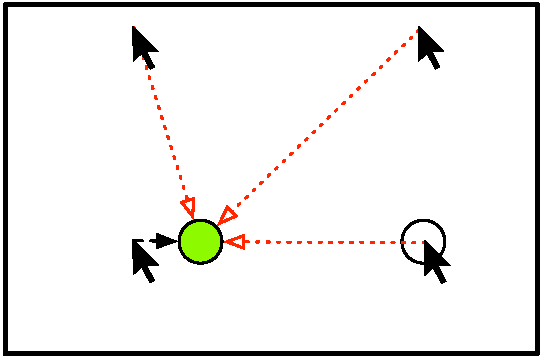
\includegraphics[width=0.9\columnwidth]{figure}
  \caption{Images should have a high resolution---preferably a vector image 
      for line-art or charts.}
  \label{fig:sample}
\end{figure}

\section{Figures and Tables}
Place figures and tables at the top or bottom of the appropriate column or
columns (try not to place them in the middle of a column), on the same page as
the relevant text (see Figure~\ref{fig:sample}). A figure or table may extend
across both columns to a maximum width of 17.78 cm (7 in.).

Captions should be Times 9-point bold. They should be numbered (e.g.,
``Table~\ref{tab:table1}'' or ``Figure~\ref{fig:sample}''), centred, and placed
beneath the figure or table. Please note that the words ``Figure'' and ``Table''
should be spelled out (e.g., ``Figure'' rather than ``Fig.'') wherever they
occur.

Tables should be formatted cleanly, with good contrast and spacing. The
\href{http://ctan.org/pkg/booktabs}{\texttt{booktabs}} package provides commands
for proper vertical spacing and horizontal rules. The
\textit{Publication Manual of the APA}~\cite{apa} has additional guidance on how
to design tables for maximum clarity. In general, limit the use of rules (lines)
to those that are necessary for clarity (and never use vertical rules), do not 
use background colours or shading, and ensure that the table can be understood
on its own.

\begin{table}
  \centering
  \begin{tabular}{ccc}
    \toprule
    & \multicolumn{2}{c}{Caption Location} \\
    \cmidrule(r){2-3}
    Object & Pre-2002 & 2003 onwards \\
    \midrule
    Tables & Above & Below \\
    Figures & Below & Below \\
    \bottomrule
  \end{tabular}
  \caption{Table captions should be placed below the table.}
  \label{tab:table1}
\end{table}

\section{Language, Style, and Content}
The written language of SIGCHI is English. Spelling and punctuation may use any
dialect of English (e.g., British, Canadian, US, etc.) provided this is done
consistently. Hyphenation is optional. To ensure suitability for an
international audience, please pay attention to the following:

\begin{itemize}
\item Write in a straightforward style.
\item Try to avoid long or complex sentence structures.
\item Briefly define or explain all technical terms that may be unfamiliar to
  readers. For example:
  \begin{itemize}
    \item Explain all acronyms the first time they are used in your text---e.g.,
      ``Digital Signal Processing (DSP)''.
    \item Explain local references (i.e., not everyone knows all city names in a
      particular country).
    \item Explain ``insider'' comments. Ensure that your whole audience
      understands any reference whose meaning you do not describe (e.g., do not
      assume that everyone has used a Macintosh or a particular application).
    \item Explain colloquial language and puns. Understanding phrases like ``red
      herring'' may require a local knowledge of English. Humour and irony are
      difficult to translate.
  \end{itemize}
\item Use unambiguous forms for culturally localised concepts, such as times,
  dates, currencies and numbers (e.g., ``1-5-97'' or ``5/1/97'' may mean 5
  January or 1 May; ``seven o'clock'' may mean 7:00 am or 19:00). For
  currencies, indicate equivalences---e.g., ``Participants were paid 1,000
  rupees, or roughly USD\$15.''
\item Be careful with the use of gender-specific pronouns (he, she) and other
  gendered words (chairman, manpower, man-months). Use inclusive language that
  is gender-neutral (e.g., she or he, they, s/he, chair, staff, staff-hours,
  person-years). Refer to the APA's
  ``\href{http://supp.apa.org/style/pubman-ch03.00.pdf}{\it Guidelines for 
  Unbiased Language}''~\cite{apa} for advice and examples regarding  gender and
  other presonal attributes.
\item If possible, use the full (extended) alphabetic character set for names of
  persons, institutions, and places (e.g., Gr{\o}nb{\ae}k, Lafreni\'ere,
  S\'anchez, Universit{\"a}t, Wei{\ss}enbach, Z{\"u}llighoven, \r{A}rhus, etc.).
  If using non-Latin characters, provide appropriate romanisation.
\end{itemize}

\section{Page Numbering, Headers, and Footers}
The \texttt{preprint} and \texttt{submission} versions of your document will
have page numbers centred in the footer. These will be removed in the
\texttt{final} version of accepted papers, as page numbers, headers, and footers
will be added by the conference printers.

\section{Producing and Testing PDF Files}
We recommend that you produce a PDF version of your submission well
before the final deadline. Your PDF file must be ACM DL Compliant. The
requirements for an ACM Compliant PDF are available at:
{\url{http://www.sheridanprinting.com/typedept/ACM-distilling-settings.htm}}.

Test your PDF file by viewing or printing it with the same software we will use
when we receive it, Adobe Acrobat~\cite{acrobat}.

\section{Blind Review}
For archival submissions, CHI requires a ``blind review''. To prepare your
submission for blind review, switch the document mode to \texttt{submission} to
remove author and institutional identities in the title and header areas of the
paper. You may also need to remove part or all of the Acknowledgments text.
Further suppression of identity in the body of the paper and references is left
to the authors' discretion. For more details, see the submission guidelines and
checklist for your submission category.

\subsection{\LaTeX\ Commands}
To assist in automatically showing or hiding regions of your document, the
commands \texttt{\textbackslash preprintonly\{...\}},
\texttt{\textbackslash sub\-mis\-sion\-only\{...\}}, and
\texttt{\textbackslash finalonly\{...\}} can be used to wrap content that should
only appear in a particular modes.

A \texttt{\textbackslash hideforsubmission\{...\}} command can be used to remove
content \texttt{submission} mode only---for example, the
\textit{Acknowledgements} section.

% Use `balance' to ensure that the columns on the last page line up. 
% Getting this to work can be a bit tricky, because the \balance command 
% must appear in the first column of the last page.
%
% If balance doesn't work for you, you can remove it and hard-code a column 
% break in the bbl file:
%     http://stackoverflow.com/questions/2149854/
%
\balance

\section{Conclusion}
It is important that you write for the SIGCHI audience. Please read previous
years' proceedings to understand the writing style and conventions that
successful authors have used.  It is particularly important that you state
clearly what you have done, not merely what you plan to do, and explain how your
work is different from previously published work, i.e., what is the unique
contribution that your work makes to the field?  Please consider what the reader
will learn from your submission, and how they will find your work useful. If you
write with these questions in mind, your work is more likely to be successful,
both in being accepted into the conference, and in influencing the work of our
field.

\section{Acknowledgments}
We thank CHI, PDC and CSCW volunteers, and all publications support and staff,
who wrote and provided helpful comments on previous versions of this document.
Some of the references cited in this paper are included for illustrative
purposes only.

\bibliography{sample}
\end{document}
